\documentclass[aspectratio=169]{beamer}

\usepackage[T1]{fontenc}
\usepackage[utf8]{inputenc}
\usepackage{lmodern}
\usepackage{microtype}
\usepackage{xcolor}
\usepackage{tikz}
\usetikzlibrary{positioning, arrows.meta}
\usepackage{booktabs}
\usepackage{fontawesome5}

\definecolor{wurgreen}{HTML}{34B233}
\definecolor{darkgreen}{HTML}{1F6B1E}
\definecolor{darknavy}{HTML}{1A1A2E}
\definecolor{midgray}{HTML}{6B7280}
\definecolor{lightgray}{HTML}{F3F4F6}
\definecolor{lightgreen}{HTML}{E8F7E8}
\definecolor{bodytext}{HTML}{1F2937}
\definecolor{warnred}{HTML}{FEE2E2}
\definecolor{warnborder}{HTML}{EF4444}

\usetheme{default}
\usecolortheme{default}
\usefonttheme{professionalfonts}
\setbeamertemplate{navigation symbols}{}
\setbeamertemplate{itemize items}{\textcolor{wurgreen}{\textbullet}}
\setbeamertemplate{itemize subitem}{\textcolor{midgray}{--}}
\setbeamercolor{frametitle}{fg=white, bg=darknavy}
\setbeamerfont{frametitle}{size=\large, series=\bfseries}
\setbeamertemplate{frametitle}{%
  \begin{beamercolorbox}[wd=\paperwidth, ht=1.1cm, dp=0.2cm, leftskip=0.6cm]{frametitle}
    \usebeamerfont{frametitle}\insertframetitle
  \end{beamercolorbox}}
\setbeamercolor{background canvas}{bg=white}
\setbeamercolor{normal text}{fg=bodytext}
\setbeamertemplate{footline}{%
  \begin{beamercolorbox}[wd=\paperwidth, ht=0.4cm, dp=0.15cm]{footline}
    \hspace{0.5cm}\textcolor{midgray}{\tiny Bags, Vectors \& Transformers · Wageningen University \& Research}%
    \hfill\textcolor{midgray}{\tiny \insertframenumber}\hspace{0.4cm}
  \end{beamercolorbox}}

\begin{document}

% ── TITLE SLIDE ──────────────────────────────────────────────────────────────
{
\setbeamertemplate{footline}{}
\begin{frame}[plain]
  \begin{tikzpicture}[remember picture, overlay]
    \fill[darknavy] (current page.south west) rectangle (current page.north east);
    \fill[wurgreen] (current page.south west) rectangle
      ([xshift=0.45cm]current page.north west);
    \node[anchor=west, text=white, font=\huge\bfseries, text width=13cm]
      at ([xshift=1.1cm, yshift=1.2cm]current page.west)
      {Bags, Vectors \& Transformers};
    \node[anchor=west, text=wurgreen, font=\large, text width=12cm]
      at ([xshift=1.1cm, yshift=0.05cm]current page.west)
      {Bag-of-Words Approaches · Day 1, Part 4};
    \node[anchor=west, text=midgray, font=\small, text width=12cm]
      at ([xshift=1.1cm, yshift=-1.5cm]current page.west)
      {Denise J. Roth, PhD Candidate\\
       Strategic Communication Group · Wageningen University \& Research};
  \end{tikzpicture}
\end{frame}
}

% ── SLIDE 1: The landscape ───────────────────────────────────────────────────
\begin{frame}{Three (Common) Ways to Analyze a Bag of Words}
\vspace{0.2cm}
{\small Once your text is a \textbf{document-term matrix}, what can you actually do
with it? Three classic families of approaches, differing mainly in \textbf{how much
they rely on the researcher versus the data}.}

\bigskip
\begin{columns}[t]
  \column{0.32\textwidth}
  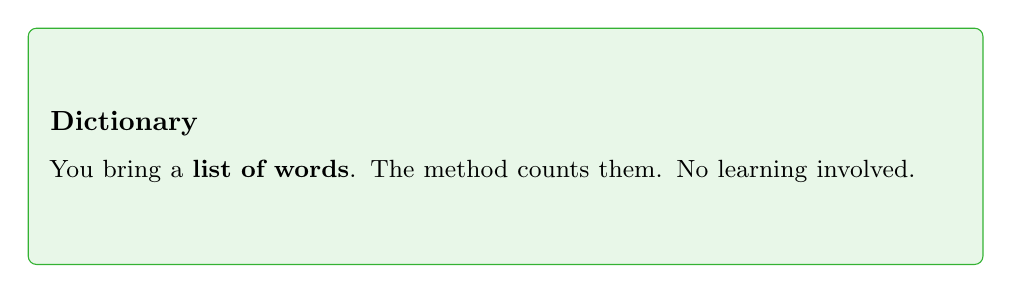
\begin{tikzpicture}
    \node[fill=lightgreen, draw=wurgreen, rounded corners=3pt,
          inner xsep=8pt, inner ysep=8pt, text width=\columnwidth-16pt, minimum height=3cm]{%
      \textbf{Dictionary}\\[5pt]
      {\small You bring a \textbf{list of words}. The method counts them. No learning involved.}};
  \end{tikzpicture}

  \column{0.32\textwidth}
  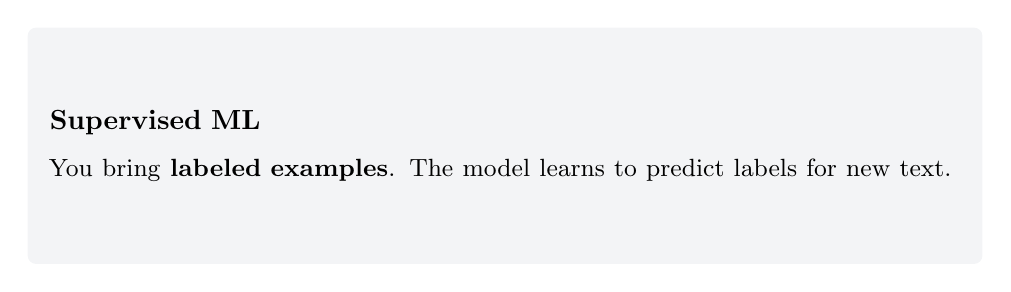
\begin{tikzpicture}
    \node[fill=lightgray, rounded corners=3pt,
          inner xsep=8pt, inner ysep=8pt, text width=\columnwidth-16pt, minimum height=3cm]{%
      \textbf{Supervised ML}\\[5pt]
      {\small You bring \textbf{labeled examples}. The model learns to predict labels for new text.}};
  \end{tikzpicture}

  \column{0.32\textwidth}
  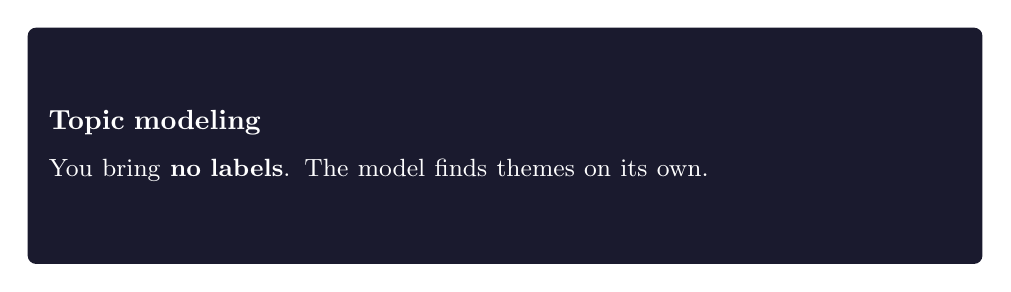
\begin{tikzpicture}
    \node[fill=darknavy, rounded corners=3pt,
          inner xsep=8pt, inner ysep=8pt, text width=\columnwidth-16pt, minimum height=3cm]{%
      \textcolor{white}{\textbf{Topic modeling}}\\[5pt]
      {\small\textcolor{white}{You bring \textbf{no labels}. The model finds themes on its own.}}};
  \end{tikzpicture}
\end{columns}
\end{frame}

% ── SLIDE 2: Supervised vs unsupervised ──────────────────────────────────────
\begin{frame}{A Key Distinction: Supervised vs.\ Unsupervised}
\vspace{0.3cm}
\begin{columns}[t]
  \column{0.48\textwidth}
  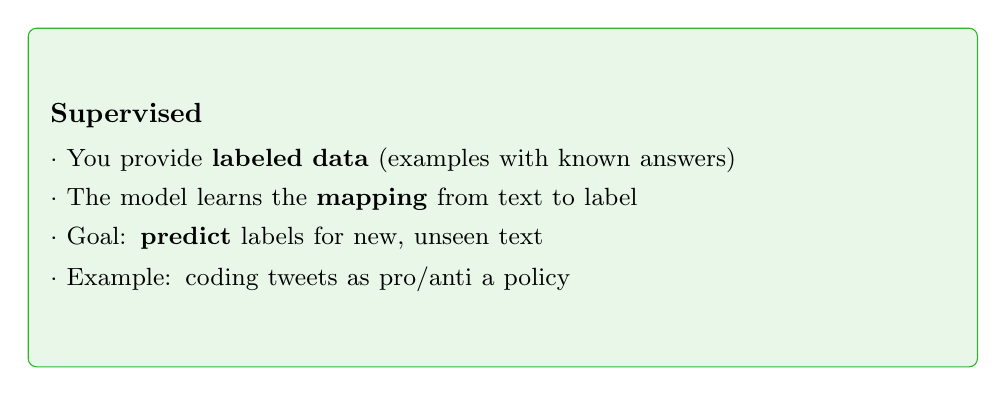
\begin{tikzpicture}
    \node[fill=lightgreen, draw=wurgreen, rounded corners=3pt,
          inner xsep=8pt, inner ysep=8pt, text width=\columnwidth-18pt, minimum height=4.3cm]{%
      \textbf{Supervised}\\[5pt]
      {\small
      $\cdot$ You provide \textbf{labeled data} (examples with known answers)\\[3pt]
      $\cdot$ The model learns the \textbf{mapping} from text to label\\[3pt]
      $\cdot$ Goal: \textbf{predict} labels for new, unseen text\\[3pt]
      $\cdot$ Example: coding tweets as pro/anti a policy}};
  \end{tikzpicture}

  \column{0.48\textwidth}
  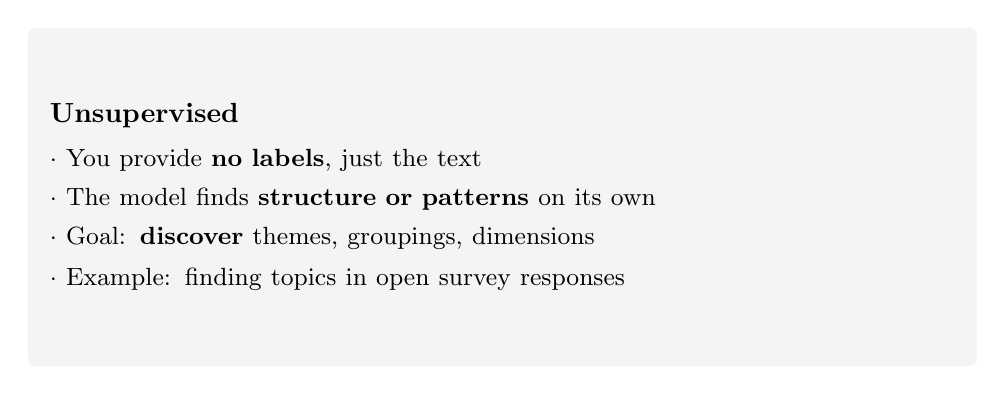
\begin{tikzpicture}
    \node[fill=lightgray, rounded corners=3pt,
          inner xsep=8pt, inner ysep=8pt, text width=\columnwidth-18pt, minimum height=4.3cm]{%
      \textbf{Unsupervised}\\[5pt]
      {\small
      $\cdot$ You provide \textbf{no labels}, just the text\\[3pt]
      $\cdot$ The model finds \textbf{structure or patterns} on its own\\[3pt]
      $\cdot$ Goal: \textbf{discover} themes, groupings, dimensions\\[3pt]
      $\cdot$ Example: finding topics in open survey responses}};
  \end{tikzpicture}
\end{columns}

\medskip
{\small\textcolor{midgray}{\textit{Dictionaries sit slightly apart: rule-based, no learning at all ---
but like supervised methods, you decide in advance what you are looking for.}}}
\end{frame}

% ── SLIDE 3: Dictionary - what it is ─────────────────────────────────────────
\begin{frame}{Approach 1: Dictionary Methods}
\vspace{0.2cm}
{\small A \textbf{dictionary} (or lexicon) is a predefined \textbf{list of words}
associated with a category. You count how often those words appear ---
that count becomes your measure.}

\medskip
\begin{columns}[T]
  \column{0.5\textwidth}
  \vspace{0pt}
  {\small\textbf{The mechanics:}}\\[4pt]
  {\small
  \textcolor{wurgreen}{\footnotesize\faCheck}~ Define categories and their word lists\\[4pt]
  \textcolor{wurgreen}{\footnotesize\faCheck}~ Count matches in each document\\[4pt]
  \textcolor{wurgreen}{\footnotesize\faCheck}~ Often normalize by document length\\[4pt]
  \textcolor{wurgreen}{\footnotesize\faCheck}~ Compare scores across documents}

  \column{0.5\textwidth}
  \vspace{0pt}
  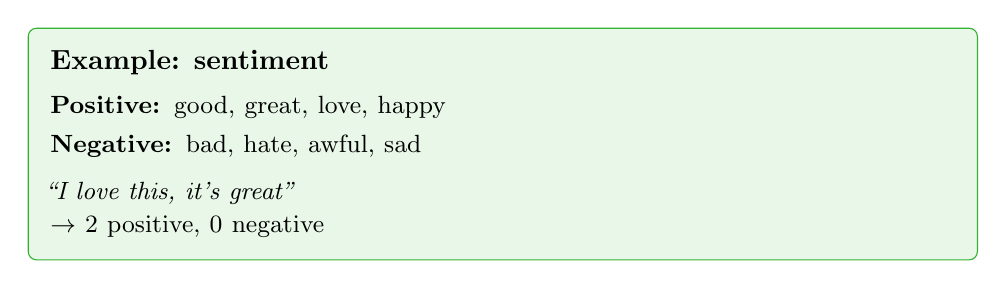
\begin{tikzpicture}
    \node[fill=lightgreen, draw=wurgreen, rounded corners=3pt,
          inner xsep=8pt, inner ysep=8pt, text width=\columnwidth-18pt]{%
      \textbf{Example: sentiment}\\[5pt]
      {\small
      \textbf{Positive:} good, great, love, happy\\[3pt]
      \textbf{Negative:} bad, hate, awful, sad\\[6pt]
      \textit{``I love this, it's great''}\\
      $\rightarrow$ 2 positive, 0 negative}};
  \end{tikzpicture}
\end{columns}
\end{frame}

% ── SLIDE 4: Dictionary - pros and cons ──────────────────────────────────────
\begin{frame}{Dictionary Methods: Pros \& Cons}
\vspace{0.3cm}
\begin{columns}[t]
  \column{0.48\textwidth}
  \begin{tikzpicture}
    \node[fill=lightgreen, draw=wurgreen, rounded corners=3pt,
          inner xsep=8pt, inner ysep=8pt, text width=\columnwidth-18pt, minimum height=4.5cm]{%
      \textcolor{darkgreen}{\textbf{\faThumbsUp\enspace Strengths}}\\[6pt]
      {\small
      $\cdot$ \textbf{Transparent} --- you see exactly what is counted\\[3pt]
      $\cdot$ \textbf{No training data} needed\\[3pt]
      $\cdot$ \textbf{Fast} and reproducible\\[3pt]
      $\cdot$ Easy to explain to reviewers\\[3pt]
      $\cdot$ Good when categories are well-defined}};
  \end{tikzpicture}

  \column{0.48\textwidth}
  \begin{tikzpicture}
    \node[fill=warnred, draw=warnborder, rounded corners=3pt,
          inner xsep=8pt, inner ysep=8pt, text width=\columnwidth-18pt, minimum height=4.5cm]{%
      \textcolor{warnborder}{\textbf{\faThumbsDown\enspace Weaknesses}}\\[6pt]
      {\small
      $\cdot$ \textbf{Context-blind} --- ``not good'' counts as positive\\[3pt]
      $\cdot$ Misses \textbf{sarcasm}, irony, negation\\[3pt]
      $\cdot$ Dictionaries are \textbf{domain-specific}\\[3pt]
      $\cdot$ Off-the-shelf lists may not fit your data\\[3pt]
      $\cdot$ Validity depends entirely on the word list}};
  \end{tikzpicture}
\end{columns}
\end{frame}

% ── SLIDE 5: Supervised ML - what it is ──────────────────────────────────────
\begin{frame}{Approach 2: Supervised Machine Learning}
\vspace{0.2cm}
{\small Instead of specifying words yourself, you give the model \textbf{labeled examples}
and let it \textbf{learn} which features (words) predict which label.}

\bigskip
\begin{center}
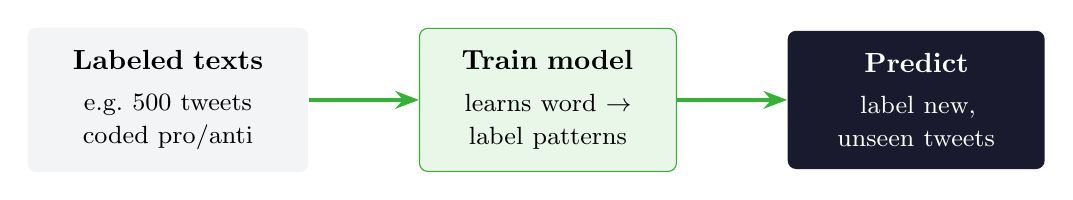
\begin{tikzpicture}[node distance=1.3cm]
  \node[fill=lightgray, rounded corners=3pt, inner sep=8pt, text width=3cm, align=center] (label)
    {\textbf{Labeled texts}\\[3pt]{\small e.g.\ 500 tweets coded pro/anti}};
  \node[fill=lightgreen, draw=wurgreen, rounded corners=3pt, inner sep=8pt,
        text width=2.7cm, align=center, right=1.4cm of label] (train)
    {\textbf{Train model}\\[3pt]{\small learns word $\rightarrow$ label patterns}};
  \node[fill=darknavy, rounded corners=3pt, inner sep=8pt,
        text width=2.7cm, align=center, right=1.4cm of train] (predict)
    {\textcolor{white}{\textbf{Predict}}\\[3pt]{\small\textcolor{white}{label new, unseen tweets}}};
  \draw[-{Stealth[length=3mm]}, wurgreen, line width=1.2pt] (label) -- (train);
  \draw[-{Stealth[length=3mm]}, wurgreen, line width=1.2pt] (train) -- (predict);
\end{tikzpicture}
\end{center}

\bigskip
{\small Common models: \textbf{Naive Bayes}, \textbf{logistic regression},
\textbf{support vector machines}. The DTM is the input; the labels are what you
are predicting. You hold out some data to \textbf{validate} accuracy.}
\end{frame}

% ── SLIDE 6: Supervised ML - pros and cons ───────────────────────────────────
\begin{frame}{Supervised ML: Pros \& Cons}
\vspace{0.3cm}
\begin{columns}[t]
  \column{0.48\textwidth}
  \begin{tikzpicture}
    \node[fill=lightgreen, draw=wurgreen, rounded corners=3pt,
          inner xsep=8pt, inner ysep=8pt, text width=\columnwidth-18pt, minimum height=4.5cm]{%
      \textcolor{darkgreen}{\textbf{\faThumbsUp\enspace Strengths}}\\[6pt]
      {\small
      $\cdot$ \textbf{Learns from your data} --- fits your domain\\[3pt]
      $\cdot$ Captures \textbf{subtle patterns} a dictionary misses\\[3pt]
      $\cdot$ \textbf{Measurable accuracy} via held-out data\\[3pt]
      $\cdot$ Scales to millions of documents once trained}};
  \end{tikzpicture}

  \column{0.48\textwidth}
  \begin{tikzpicture}
    \node[fill=warnred, draw=warnborder, rounded corners=3pt,
          inner xsep=8pt, inner ysep=8pt, text width=\columnwidth-18pt, minimum height=4.5cm]{%
      \textcolor{warnborder}{\textbf{\faThumbsDown\enspace Weaknesses}}\\[6pt]
      {\small
      $\cdot$ Needs \textbf{labeled training data} (costly to make)\\[3pt]
      $\cdot$ Labels must be \textbf{reliable} and consistent\\[3pt]
      $\cdot$ Can \textbf{overfit} or learn spurious cues\\[3pt]
      $\cdot$ Less transparent --- more of a ``black box''}};
  \end{tikzpicture}
\end{columns}
\end{frame}

% ── SLIDE 7: Topic modeling - what it is ─────────────────────────────────────
\begin{frame}{Approach 3: Topic Modeling}
\vspace{0.2cm}
{\small \textbf{Topic modeling} is \textbf{unsupervised}: you give it only the text,
and it discovers clusters of words that tend to \textbf{co-occur} --- which we
interpret as \textbf{topics}. The most common method is \textbf{LDA}
(Latent Dirichlet Allocation).}

\medskip
\begin{columns}[T]
  \column{0.5\textwidth}
  \vspace{0pt}
  {\small\textbf{The core intuition:}}\\[4pt]
  {\small
  \textcolor{wurgreen}{$\cdot$} Each \textbf{document} is a mixture of topics\\[4pt]
  \textcolor{wurgreen}{$\cdot$} Each \textbf{topic} is a distribution over words\\[4pt]
  \textcolor{wurgreen}{$\cdot$} The model infers both from co-occurrence\\[4pt]
  \textcolor{wurgreen}{$\cdot$} You \textbf{interpret and label} the topics}

  \column{0.5\textwidth}
  \vspace{0pt}
  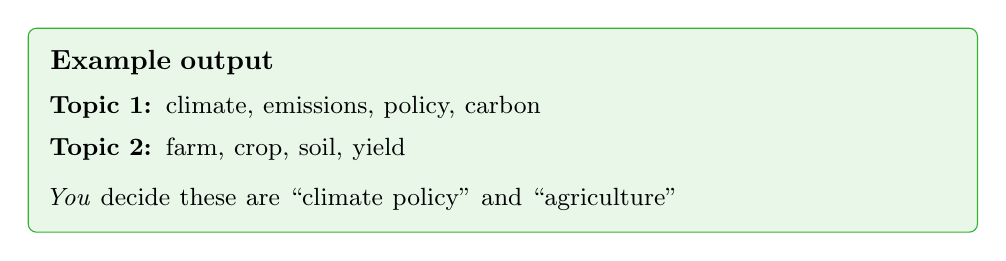
\begin{tikzpicture}
    \node[fill=lightgreen, draw=wurgreen, rounded corners=3pt,
          inner xsep=8pt, inner ysep=8pt, text width=\columnwidth-18pt]{%
      \textbf{Example output}\\[5pt]
      {\small
      \textbf{Topic 1:} climate, emissions, policy, carbon\\[4pt]
      \textbf{Topic 2:} farm, crop, soil, yield\\[6pt]
      \textit{You} decide these are ``climate policy'' and ``agriculture''}};
  \end{tikzpicture}
\end{columns}
\end{frame}

% ── SLIDE 8: Topic modeling - pros and cons ──────────────────────────────────
\begin{frame}{Topic Modeling: Pros \& Cons}
\vspace{0.3cm}
\begin{columns}[t]
  \column{0.48\textwidth}
  \begin{tikzpicture}
    \node[fill=lightgreen, draw=wurgreen, rounded corners=3pt,
          inner xsep=8pt, inner ysep=8pt, text width=\columnwidth-18pt, minimum height=4.6cm]{%
      \textcolor{darkgreen}{\textbf{\faThumbsUp\enspace Strengths}}\\[6pt]
      {\small
      $\cdot$ \textbf{No labeling} required\\[3pt]
      $\cdot$ Great for \textbf{exploration} of large corpora\\[3pt]
      $\cdot$ Surfaces themes you \textbf{did not anticipate}\\[3pt]
      $\cdot$ Handles many topics at once\\[3pt]
      $\cdot$ Good first pass on unfamiliar data}};
  \end{tikzpicture}

  \column{0.48\textwidth}
  \begin{tikzpicture}
    \node[fill=warnred, draw=warnborder, rounded corners=3pt,
          inner xsep=8pt, inner ysep=8pt, text width=\columnwidth-18pt, minimum height=4.6cm]{%
      \textcolor{warnborder}{\textbf{\faThumbsDown\enspace Weaknesses}}\\[6pt]
      {\small
      $\cdot$ You must \textbf{choose the number of topics}\\[3pt]
      $\cdot$ Topics can be \textbf{incoherent} or hard to label\\[3pt]
      $\cdot$ Results can be \textbf{unstable} across runs\\[3pt]
      $\cdot$ \textbf{Interpretation} is subjective\\[3pt]
      $\cdot$ Validation is genuinely hard}};
  \end{tikzpicture}
\end{columns}
\end{frame}

% ── SLIDE 9: Comparison table ────────────────────────────────────────────────
\begin{frame}{Putting It Together}
\vspace{0.3cm}
\begin{center}
\renewcommand{\arraystretch}{1.5}
{\small
\begin{tabular}{p{2.4cm}|p{2.6cm}p{2.6cm}p{2.6cm}}
 & \textbf{Dictionary} & \textbf{Supervised ML} & \textbf{Topic modeling} \\
\hline
\textbf{Learning} & None (rule-based) & Supervised & Unsupervised \\
\textbf{You provide} & A word list & Labeled examples & Just the text \\
\textbf{Best for} & Known categories & Predicting labels & Exploring themes \\
\textbf{Main risk} & Context-blind & Needs good labels & Hard to interpret \\
\end{tabular}
}
\end{center}

\bigskip
{\small\textcolor{midgray}{\textit{These are not rivals --- researchers often combine them.
A topic model to explore, a dictionary to measure, a classifier to scale.}}}
\end{frame}

% ── SLIDE 10: Which to choose ────────────────────────────────────────────────
\begin{frame}{Which Should You Use?}
\vspace{0.3cm}
\begin{itemize}\setlength\itemsep{10pt}
  \item[\textcolor{wurgreen}{\faArrowRight}]
    \textbf{Know exactly what you're measuring} and have clear categories?
    Start with a \textbf{dictionary}.
  \item[\textcolor{wurgreen}{\faArrowRight}]
    \textbf{Have (or can create) labeled data} and want to predict a category?
    Use \textbf{supervised ML}.
  \item[\textcolor{wurgreen}{\faArrowRight}]
    \textbf{Not sure what's in your corpus} and want to explore?
    Try \textbf{topic modeling}.
\end{itemize}

\bigskip
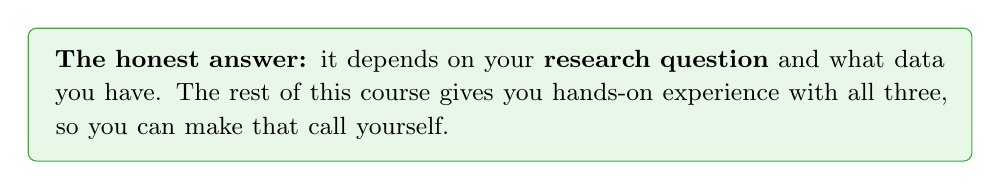
\begin{tikzpicture}
  \node[fill=lightgreen, draw=wurgreen, rounded corners=3pt,
        inner xsep=10pt, inner ysep=8pt, text width=\textwidth-24pt]{%
    {\small\textbf{The honest answer:} it depends on your \textbf{research question}
    and what data you have. The rest of this course gives you hands-on experience
    with all three, so you can make that call yourself.}};
\end{tikzpicture}
\end{frame}

\end{document}
